\documentclass{acm_proc_article-sp}
\usepackage{subfiles}

\usepackage[italian]{babel}
\usepackage[utf8]{inputenc}
\usepackage{url}
\usepackage{enumitem}


\begin{document}

\title{Reminiscens, una knowledge base di risorse storiche per supportare la reminiscenza}
\subtitle{Tesi di laurea triennale}
 

\numberofauthors{1} %  in this sample file, there are a *total*
% of EIGHT authors. SIX appear on the 'first-page' (for formatting
% reasons) and the remaining two appear in the \additionalauthors section.
%
\author{
% 1st. author
\alignauthor
Nicola Parrello\\
       \affaddr{Università degli studi di Trento}\\
       \affaddr{Via Sommarive, 14}\\
       \affaddr{38123 Povo (Trento)}\\
       \email{parrello.nicola@gmail.com}
}
\maketitle
\subfile{abstract}

\subfile{intro}

\begin{figure*}[t]
\centering
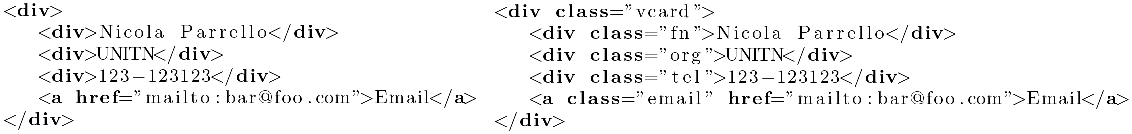
\includegraphics[width=1.0\textwidth]{microformats.pdf}
\caption{Un contatto senza e con il microformato hCard}
\label{fig:microformats}
\end{figure*}

\subfile{problem}

\begin{figure*}[t]
\centering
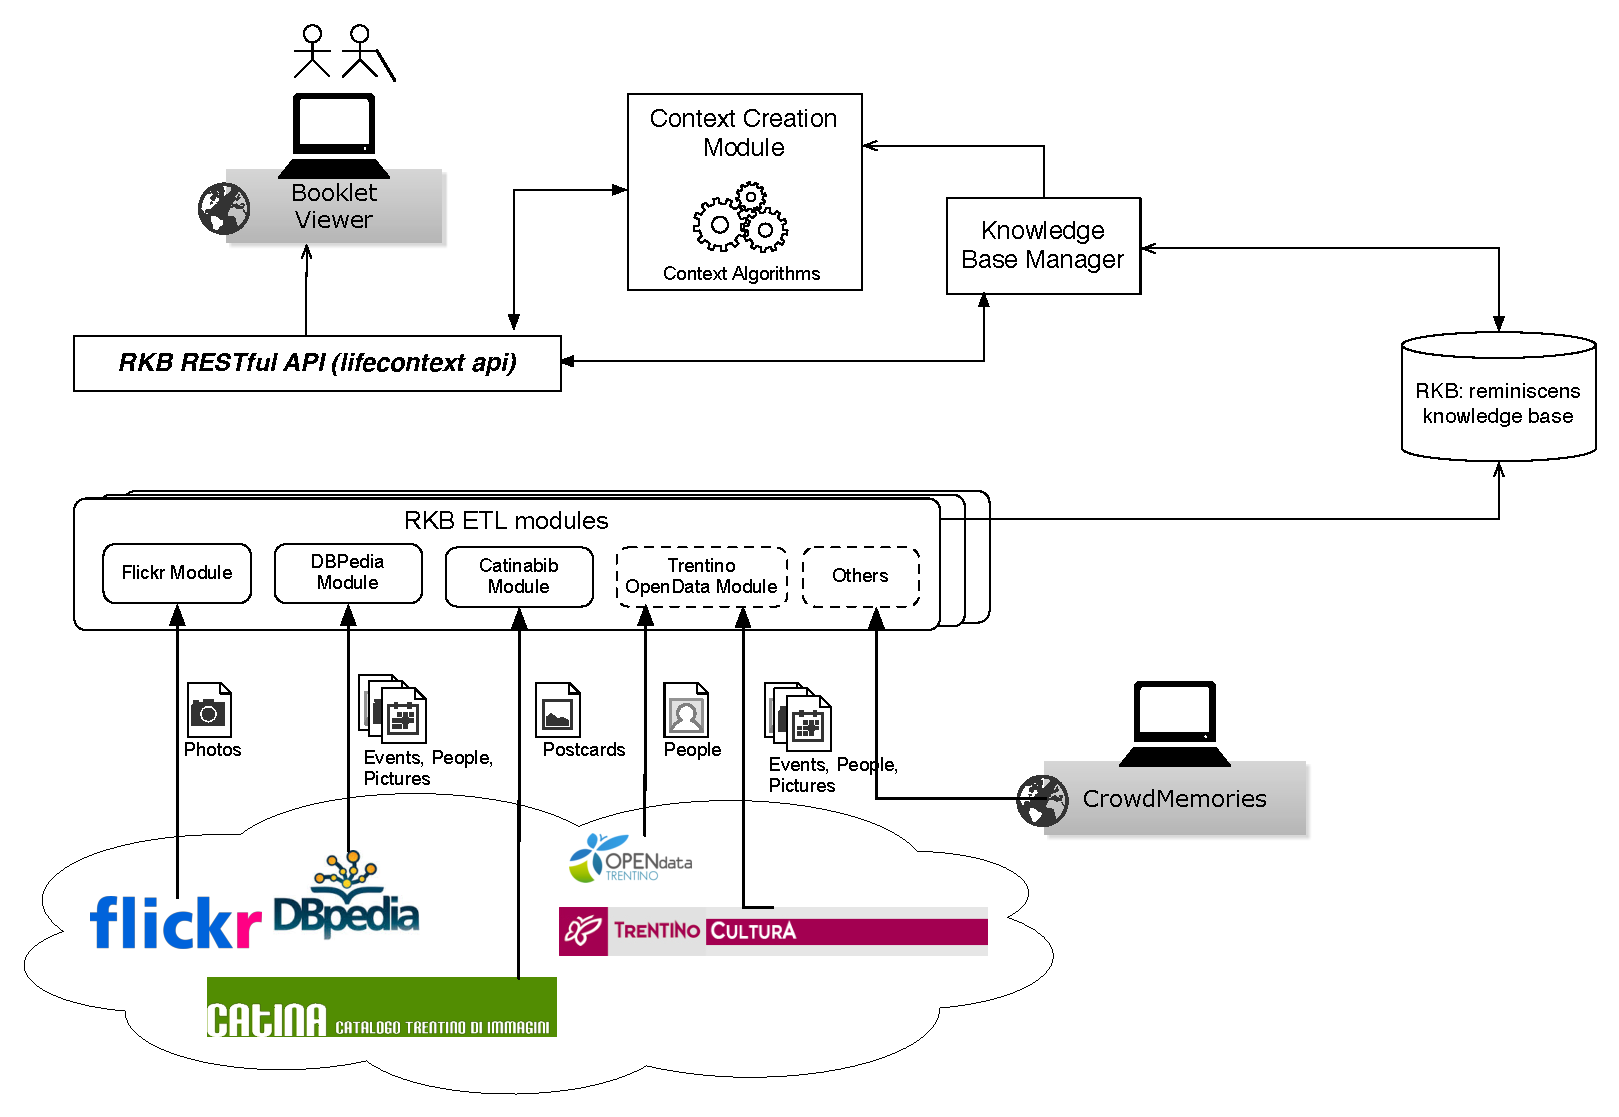
\includegraphics[width=1.0\textwidth]{architecture.pdf}
\caption{Architettura di Reminiscens}
\label{fig:architecture}
\end{figure*}

\subfile{sota}

\begin{figure*}[t]
\centering
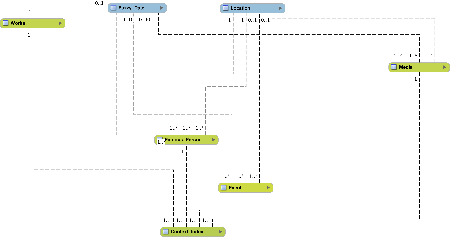
\includegraphics[width=1.0\textwidth]{model.pdf}
\caption{Architettura della Knowledge Base}
\label{fig:model}
\end{figure*}

\begin{figure*}[t]
\centering
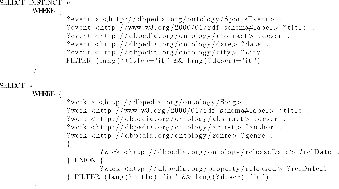
\includegraphics[width=1.0\textwidth]{sparql.pdf}
\caption{Alcune query SPARQL}
\label{fig:sparql}
\end{figure*}

\begin{figure*}[t]
\centering
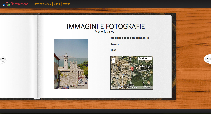
\includegraphics[width=1.0\textwidth]{booklet.pdf}
\caption{Una pagina del Booklet, ottenuto con query 1990 - Trento}
\label{fig:booklet}
\end{figure*}

\subfile{solution}

\begin{table}
\parbox{.45\linewidth}{
\centering
\begin{tabular}{|r|l|}
\hline
Tipo & Numero \\
\hline
Immagini & 548 \\
Canzoni & 1587 \\
Eventi & 630 \\
Persone famose & 479 \\
\hline
\end{tabular}
\caption{Tipi raccolti}
\label{tab:entitykind}
}
\hfill
\parbox{.45\linewidth}{
\centering
\begin{tabular}{|r|l|}
\hline
Sorgente & Numero \\
\hline
Flickr & 340 \\
DBpedia & 1168 \\
Catinabib & 208 \\
OpenData Trentino & 463 \\
Crowd e altro & 1065 \\
\hline
\end{tabular}
\caption{Distribuzione delle sorgenti}
\label{tab:entitysource}
}
\end{table}

\subfile{conclusions}
%\end{document}  % This is where a 'short' article might terminate

%ACKNOWLEDGMENTS are optional
\section{Riconoscimenti}
Ringrazio il mio relatore Prof. Fabio Casati, il correlatore Cristhian Parra e LifeParticipation\footnote{\url{http://www.lifeparticipation.org/}} per avermi seguito durante tutto il percorso dell'internship che ha portato a questa tesi e al lavoro da me fatto. Ringraziamenti estesi a Manuel Cattin Cosso e chi mi ha sopportato nei momenti di stress di quest'anno.

%
% The following two commands are all you need in the
% initial runs of your .tex file to
% produce the bibliography for the citations in your paper.
\bibliographystyle{abbrv}
\bibliography{sigproc}  % sigproc.bib is the name of the Bibliography in this case
% You must have a proper ".bib" file
%  and remember to run:
% latex bibtex latex latex
% to resolve all references
%
% ACM needs 'a single self-contained file'!
%
%APPENDICES are optional
%\balancecolumns
\appendix
%Appendix A
\subfile{appendix_booklet}

\subfile{appendix_apidocs}



\balancecolumns
% That's all folks!
\end{document}
